\chapter{A Different Way Of Living}

This chapter follows J. Krishnamurti's dialogue with Alan W. Anderson on living, love, death, and consciousness. The lecture has no blackboard derivation to reproduce. Its rigor lies elsewhere: in the care with which it separates conflict from perception, escape from inquiry, thought from its proper use, and belief from immediate action. We will use compact formulas and diagrams only as aids to the argument, not as substitutes for the spoken inquiry.

\section{The Question Resumed: Living, Love, Death}

Anderson opens by recalling the unfinished question from the previous conversation: the relation among living, love, and death. Krishnamurti accepts the triad, but he does not begin with death as a future event or with love as an ideal. He first asks what we actually call living.

That order matters. If living is already disorderly, frightened, and divided, then any answer about love or death that grows out of that disorder will merely extend it. The inquiry must begin where we are.

We may write the first movement as:
\begin{equation}
\text{living} \longrightarrow \text{love} \longrightarrow \text{death}.
\end{equation}
This is not a chronological sequence. It is the order of investigation. We begin with the fact of daily life, because that is the ground from which our questions about love and death arise.

Krishnamurti's opening description of living is intentionally plain. Living is not introduced as a noble concept. It is work, relationship, ambition, economic pressure, social comparison, frustration, routine, holiday escape, violence, despair, and the persistent effort to become something more secure or more successful than what one is. The word that gathers the description is battle.

\section{What We Call Living}

The first sustained movement of the lecture is a survey of ordinary existence. Krishnamurti moves from relationship to economics, from social morality to religious escape, from office life to holidays, from the need to be successful to the need to get away. The examples are not incidental. They show the same pattern repeating in different costumes.

A compact map of the first diagnosis is:
\begin{equation}
\text{ordinary living}
   \longrightarrow
\{\text{struggle},\ \text{suffering},\ \text{frustration},\ \text{violence},\ \text{escape}\}.
\end{equation}

The holiday example is especially sharp. A person may spend decades in an office or factory and then rush through museums, countries, costumes, and spiritual atmospheres as an escape from monotony. But the escape is still organized by the same life from which it flees. The form changes; the structure remains.

Anderson then names the assumption that most people do not question: life is a battle. The usual problem is how to fight better, how to suffer less damage, how to succeed with less strain. Krishnamurti shifts the question. He does not ask how to improve the battle. He asks whether battle is living.

\subsection{Question \& Answer}

\paragraph{Question.}
Must life be a battle? Is struggle simply natural, inherited from the animal, and therefore unavoidable?

\paragraph{Answer.}
Krishnamurti's answer is to question the whole analogy. To study animal danger and then explain human conflict by it is already to confuse two things. Danger may call for immediate response; psychological conflict is something else. The human problem is not merely survival in the presence of danger. It is the inward and outward division that turns life into continuous battle.

The turn can be written:
\begin{equation}
\text{How can battle be managed?}
   \quad \longrightarrow \quad
\text{Can battle end?}
\end{equation}

This is the first decisive displacement in the lecture. We are no longer inside the problem of better conflict. We are asking whether conflict is necessary at all.

\section{Fragmentation And Perception}

Once battle is placed in question, Krishnamurti looks for its structure. Conflict means division. It means opposites, ``you'' and ``me,'' ``we'' and ``they,'' nation against nation, class against class, one inward fragment against another. Where there is fragmentation, there must be battle.

The diagnostic chain is:
\begin{equation}
\text{division}
   \longrightarrow
\text{fragmentation}
   \longrightarrow
\text{conflict}
   \longrightarrow
\text{battle}.
\end{equation}

This chain is the spine of the first half of the lecture. It keeps the inquiry from becoming sentimental. Peace is not being proposed as a pleasant ideal. The structure of conflict is being examined.

Krishnamurti then refuses a common solution. The answer is not to integrate the fragments. Integration still begins with the fragments as separate pieces and asks how to arrange them. The lecture turns instead toward perception.

\begin{definition}
In this chapter, \emph{perception} means direct seeing of what is taking place, without a separate observer trying to change, condemn, justify, suppress, or integrate what is seen.
\end{definition}

That gives us the counter-movement:
\begin{equation}
\text{seeing what is}
   \longrightarrow
\text{perception}
   \longrightarrow
\text{action}.
\end{equation}

Here action is not a delayed conclusion. It is not method applied after analysis. The point of the phrase ``seeing acting'' is that perception and action are not separated by a psychological interval in which the observer decides what to do.

\subsection{A Worked Derivation: From Division To Battle}

We can state the lecture's reasoning as a compact derivation. It is not a formal theorem, but it has a useful logical form.

\begin{enumerate}
\item Suppose daily life is organized by division: me and you, us and them, success and failure, one inward demand against another.
\item Division gives each side the character of a fragment.
\item A fragment seeks security, continuity, power, or dominance.
\item When fragments meet as rivals, the relation is conflict.
\item When conflict becomes the accepted pattern of living, life appears as battle.
\item Therefore battle is not accidental if division remains operative.
\end{enumerate}

Introduce the shorthand:
\begin{align}
D &:= \text{division},\\
F &:= \text{fragmentation},\\
C &:= \text{conflict},\\
B &:= \text{battle}.
\end{align}
Then the lecture's diagnostic chain is:
\begin{equation}
D \longrightarrow F \longrightarrow C \longrightarrow B.
\end{equation}

The important question is where this chain can be interrupted. Krishnamurti does not propose that one fragment defeat the others. He proposes that the movement of fragmentation be seen. That seeing is already the beginning of a different action.

\section{Two Energies}

The next pivot comes through Anderson's attention to the word energy. Krishnamurti speaks of energy in relation to conflict and also in relation to perception. Anderson asks, in effect, whether the energy is different at the root. Krishnamurti's clarification is that the phenomenon is different.

We introduce the following notation only as a reading aid:
\begin{align}
E_{\mathrm{conflict}} &:= \text{energy released through conflict},\\
E_{\mathrm{perception}} &:= \text{energy released through perception and action}.
\end{align}
These are not physical variables. They help us preserve the distinction in the dialogue.

The contrast is:
\begin{align}
E_{\mathrm{conflict}}
   &\longrightarrow
   \{\text{fragmentary},\ \text{divisive},\ \text{destructive},\ \text{violent}\},\\
E_{\mathrm{perception}}
   &\longrightarrow
   \{\text{non-fragmentary},\ \text{whole},\ \text{sane},\ \text{healthy}\}.
\end{align}

Anderson gives the shattering, fragmentary release of energy a strong name: demonic. Krishnamurti accepts the force of the description, but the chapter should keep the emphasis on the distinction itself. Conflict releases one kind of movement; perception releases another.

\begin{figure}
\centering
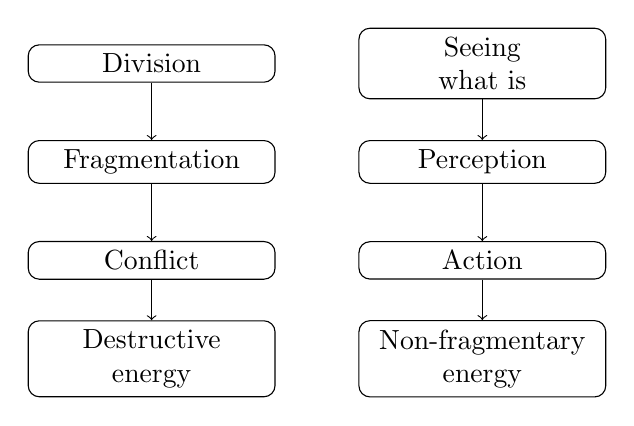
\begin{tikzpicture}[x=1cm,y=1cm]
\node[draw, rounded corners, align=center, text width=2.9cm] (d) at (0,0) {Division};
\node[draw, rounded corners, align=center, text width=2.9cm] (f) at (0,-1.25) {Fragmentation};
\node[draw, rounded corners, align=center, text width=2.9cm] (c) at (0,-2.5) {Conflict};
\node[draw, rounded corners, align=center, text width=2.9cm] (e) at (0,-3.75) {Destructive\\energy};

\node[draw, rounded corners, align=center, text width=2.9cm] (s) at (4.2,0) {Seeing\\what is};
\node[draw, rounded corners, align=center, text width=2.9cm] (p) at (4.2,-1.25) {Perception};
\node[draw, rounded corners, align=center, text width=2.9cm] (a) at (4.2,-2.5) {Action};
\node[draw, rounded corners, align=center, text width=2.9cm] (w) at (4.2,-3.75) {Non-fragmentary\\energy};

\draw[->] (d) -- (f);
\draw[->] (f) -- (c);
\draw[->] (c) -- (e);

\draw[->] (s) -- (p);
\draw[->] (p) -- (a);
\draw[->] (a) -- (w);
\end{tikzpicture}
\caption{A compact map of the lecture's contrast between conflict and perception.}
\end{figure}

The diagram is deliberately narrow. It is not a system imposed on the lecture. It is a way of keeping the two movements separate on the page.

\section{Education As The Test Case}

The dialogue then becomes practical. If a different way of living is possible, how is it to be communicated? Anderson raises the educational problem. Perhaps the teacher must first be without conflict before teaching freedom from conflict. Krishnamurti rejects the delay hidden in that assumption.

\subsection{Question \& Answer}

\paragraph{Question.}
Must the teacher first be transformed before teaching?

\paragraph{Answer.}
If the teacher waits until he is entirely free of conflict, he may wait indefinitely. Krishnamurti proposes another beginning. The teacher lives in conflict; the students live in conflict. Let that fact be acknowledged. Let both look at it together in the relationship of teaching.

The relational update is:
\begin{equation}
(\text{teacher in conflict},\ \text{student in conflict})
   \longrightarrow
\text{shared observation of conflict}.
\end{equation}

This is one of the most practical moments in the lecture. Teaching does not begin with authority claiming completion. It begins with the fact both sides share.

Anderson then adds an important caution about thought and knowledge. The dialogue must not be misunderstood to mean that thought is a disease or that knowledge is corrupt in itself. Krishnamurti accepts the correction. A microphone is a microphone; a text is a text. Thought and knowledge have proper uses. The disorder begins when thought becomes the instrument of division, self-importance, imitation, authority, or escape.

Thus the educational passage has two functions. It shows how inquiry can begin in actual relationship, and it protects the lecture from a false anti-intellectual reading. The problem is not knowledge as such. The problem is the self's use of knowledge as division.

\section{Love, The Field, And The End Of Separation}

The lecture now returns to love. If life is battle, where can love enter? If I am competing with you, trying to surpass you, using you, or resisting you, love is not being hidden by a lack of sentiment. It has no ground in that movement.

The negative statement is:
\begin{equation}
\text{battle}
   \longrightarrow
\text{no ground for love}.
\end{equation}

The positive statement is more delicate:
\begin{equation}
\text{perceiver} = \text{perceived}
   \quad \longrightarrow \quad
\text{action without psychological separation}.
\end{equation}
This identity-like expression must be read with care. It does not deny ordinary perception of objects. It points to the absence of a separate psychological observer who stands apart from what is seen and then tries to manipulate it.

Anderson's classroom example from the Gita sharpens the point. He had previously tried to show students that the field was one, not two. But now he sees that even that can remain verbal. It is one thing to explain the unity of a field. It is another to begin with the actual classroom as the field and look together.

\begin{remark}
The classroom is not an illustration added from outside. It is the practical form of the inquiry. If the classroom is the field, then the inquiry begins before doctrine, before interpretation, and before the teacher assumes the position of one who already knows.
\end{remark}

The movement can be summarized:
\begin{equation}
\text{verbal assertion of unity}
   \longrightarrow
\text{shared perception in the field}.
\end{equation}

Love, then, is not treated as an emotion to cultivate. It appears in the lecture with care, responsibility, compassion, and the ending of separation in action.

\section{Consciousness, Death, And Postponement}

Only after living and love have been examined does Krishnamurti move toward death. He says that living, love, and death are not three separate things. They are one movement.

\begin{equation}
\text{living},\ \text{love},\ \text{death}
   \longrightarrow
\text{one non-divisive movement}.
\end{equation}

But even now he does not begin with an answer about death. He first asks what consciousness is. The answer is intentionally simple:
\begin{equation}
\text{consciousness} = \text{content}.
\end{equation}

The content includes thoughts, anxieties, identifications, conflicts, attachments, detachments, fears, pleasures, agony, suffering, beliefs, and neurotic actions. A compact notation is useful if we keep it provisional:
\begin{equation}
\text{content}(\text{consciousness})
=
\{\text{thought},\ \text{anxiety},\ \text{identification},\ \text{fear},\ \text{pleasure},\ \text{suffering},\ \text{belief}\}.
\end{equation}
The set is not exhaustive. It is a compressed reminder of the spoken list.

Krishnamurti then says that this content is common. The details vary, but the structure is shared. My attachments and fears may have different objects from yours, but attachment and fear are not private inventions. In that sense the world is not outside me as an unrelated abstraction. The content of consciousness is the human field.

From here the question of death becomes exact:
\begin{equation}
\text{death}
=
\begin{cases}
\text{ending of consciousness with its content},\\
\text{continuity of consciousness with its content}.
\end{cases}
\end{equation}

Krishnamurti next examines the comfort offered by belief in continuity. If one is frightened by death, a promise of life after death can be accepted eagerly. Reincarnation enters the dialogue here, and he keeps the word karma very simple: it means action. The crucial point is not a survey of doctrine. It is the practical effect of belief.

The chain is:
\begin{equation}
\text{fear of death}
   \longrightarrow
\text{belief in continuity}
   \longrightarrow
\text{comfort}
   \longrightarrow
\text{postponement}.
\end{equation}

And postponement contradicts the immediacy that has governed the whole conversation:
\begin{equation}
\text{postponement}
   \longrightarrow
\text{contradiction of immediate action}.
\end{equation}

\subsection{Question \& Answer}

\paragraph{Question.}
If consciousness continues, can fundamental action be postponed?

\paragraph{Answer.}
That is the danger Krishnamurti exposes. The belief may say, ``behave now,'' but it may also imply that there is always another chance. Then one can stall, continue, misbehave, and take comfort in the idea of later correction. For Krishnamurti, this is not action. It is delay disguised as belief.

The lecture therefore ends not with a completed doctrine of death, but with a sharper demand. If karma means action, then the question is action now, not postponement under the cover of continuity.

\section{Summary}

The chapter has followed one continuous movement. It began with living as it is ordinarily known: conflict, struggle, escape, and battle. It then asked whether battle is necessary, and traced battle back to division and fragmentation.

The central diagnostic chain was:
\begin{equation}
D \longrightarrow F \longrightarrow C \longrightarrow B,
\end{equation}
where division gives rise to fragmentation, fragmentation gives rise to conflict, and conflict becomes the accepted battle of living.

Against that movement the lecture set another:
\begin{equation}
\text{seeing what is}
   \longrightarrow
\text{perception}
   \longrightarrow
\text{action}.
\end{equation}
The action of conflict and the action of perception are not the same:
\begin{equation}
\text{action}_{\mathrm{conflict}}
   \neq
\text{action}_{\mathrm{perception}}.
\end{equation}

The educational passage made the inquiry concrete. Teacher and student do not wait for perfection. They begin with the shared fact of conflict and look together. The love passage then showed why battle and compassion cannot occupy the same ground.

The final movement opened death through consciousness. Consciousness is its content, that content is common, and belief in continuity can become postponement. The conversation therefore leaves us with the same pressure with which it began: not theory, not comfort, not delay, but the immediate seeing of what is and the action that follows from it.